\chapter{ПРОЕКТИРОВАНИЕ СИСТЕМЫ АВТОМАТИЗАЦИИ УПРАВЛЕНИЯ ЖИЗНЕННЫМ ЦИКЛОМ ВЕБ-СЕРВИСА}
\label{cha:design}

\section{Анализ требований к системе}

Веб-сервис представляет приложение на базе архитектуры <<Клиент-Сервер>>.
Пользователь получает доступ к сервису посредством веб-браузера, запрашивающего HTML страницу у SSR сервиса web-client,
содержание которой зависит от сервиса api.
В этих двух сервисах используется общая библиотека исходного кода common.
В качестве хранилища данных используется СУБД PostgreSQL 14.1.
Данная развёртка представлена на рисунке \ref{fig:deploy-diagram}.

\begin{figure}[ht]
    \centering
    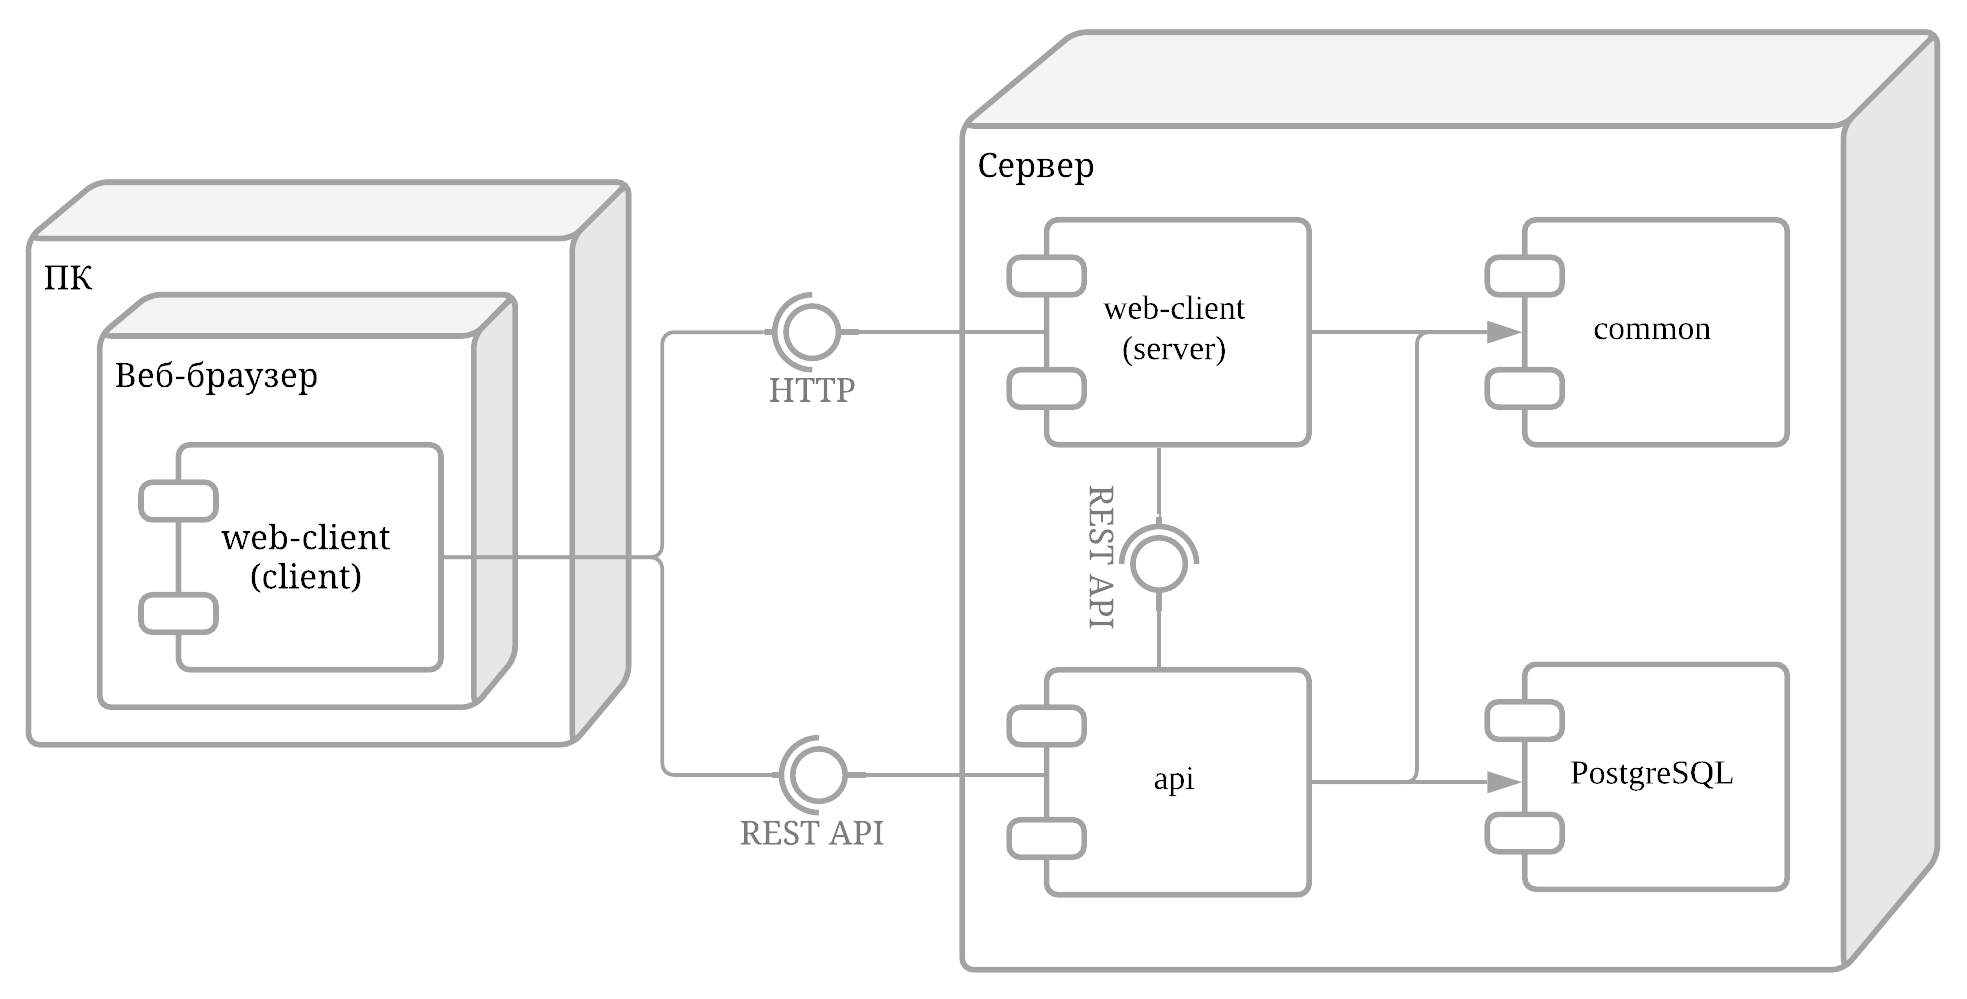
\includegraphics[scale=0.225]{src/figures/deploy-diagram}
    \caption{Диаграмма развёртывания веб-сервиса}
    \label{fig:deploy-diagram}
\end{figure}

Так как полученный для развёртывания веб-сервис базируется на Node.js и исходный код разбит на библиотеки, то для работы системы потребуется регистр Node пакетов.
Так же необходимым будет регистр Docker образов.

Согласно требованиям были сформулированы основные действующими лица (актёры) в работе системы:
\begin{itemize}
    \item администратор --- пользователь системы имеющий доступ к конфигурациям прав доступа
        и развёртывания веб-сервиса,
    \item разработчик --- пользователь системы имеющий доступ к репозиториям с исходным кодом,
        хранилищам пакетов и контейнеров, а так же управлению релизами веб-сервиса,
    \item сотрудник отдела качества (тестировщик) --- пользователь системы имеющий доступ к просмотру аналитических данных и
        проведению автоматизированных тестовых сценариев внутри заранее подготовленных окружений.
\end{itemize}

Пользователь системы подразумевает любого актёра.
На основании описания актёров и их основных возможностей была составлена диаграмма случаев использования.
Изображение данной диаграммы представлено на Рисунке \ref{fig:use-cases}.

\begin{figure}[h!]
    \centering
    \begin{tikzpicture}
        \begin{umlsystem}[x=5]{system}{Система}
            \umlusecase[width=3cm]{Управление правами доступа}
            \umlusecase[y=-4, width=3cm]{Управление развёрткой}
            \umlusecase[x=6, y=-2, width=3cm]{Конфигурация окружений}
            \umlusecase[x=6, y=-6, width=3cm]{Конфигурация системных ограничений}

            \umlusecase[y=-8, width=3cm]{Получение доступа к исходному коду и хранилищам}
            \umlusecase[y=-12, width=3cm]{Управление релизами сервиса и библиотек}

            \umlusecase[x=6, y=-14, width=3cm]{Тестирование веб-сервиса}
            \umlusecase[y=-16, width=3cm]{Сбор аналитических данных}
        \end{umlsystem}

        \umlactor[y=-2]{Администратор}{admin}
        \umlactor[y=-10]{Разработчик}{developer}
        \umlactor[y=-14]{Тестировщик}{qa}

        \umlassoc{admin}{usecase-1}
        \umlassoc{admin}{usecase-2}
        \umlassoc{developer}{usecase-5}
        \umlassoc{developer}{usecase-6}
        \umlassoc{qa}{usecase-7}
        \umlassoc{qa}{usecase-8}

        \umlinclude{usecase-3}{usecase-2}
        \umlinclude{usecase-4}{usecase-2}
    \end{tikzpicture}
    \caption{Диаграмма случаев использования системы}
    \label{fig:use-cases}
\end{figure}

Согласно требованиям системой должно поддерживаться три основных рабочих окружения веб-сервиса под различные цели:

\begin{itemize}
    \item develop --- инсценировка рабочего окружения веб-сервиса для разработчиков,
    \item testing --- окружение для проведения ручного тестирования и сбора аналитических данных,
    \item release --- рабочее окружение веб-сервиса для реальных пользователей.
\end{itemize}

С точки зрения CI/CD взаимодействие пользователя с системой сосредоточено вокруг коммита (Commit) в репозиторий и
автоматическим запуском одной или нескольких задач (Jobs) внутри определённой линии (Pipeline)\cite{cd}.
Каждая задача является набором последовательно исполняемых инструкций ожидаемо завершённых без ошибок.
В случае ошибки выполнение всей линии завершается и повторяется только по запросу пользователя.
При этом линии задач строятся динамически в зависимости от конкретного репозитория и ветки.
Результатами работы линий являются артефакты, которые содержат основную информацию о результатах работы задачи.
Данное поведение системы в общем виде отражено на Рисунке \ref{fig:system-common}.

\begin{figure}[h!]
    \centering
    \begin{tikzpicture}
        \begin{umlseqdiag}
            \umlactor[class=А]{Пользователь}{a}
            \umldatabase[class=B]{Репозиторий}{b}
            \umlobject[class=C]{Линия}{c}
            \umlobject[class=D]{Задача}{d}
            \begin{umlcall}[op=коммит, type=asynchron]{a}{b}
                \begin{umlcall}[op=запускает, type=asynchron]{b}{c}
                    \begin{umlcall}[op=выполняет, type=synchron, return=0]{c}{d}
                    \end{umlcall}
                    \begin{umlcall}[op=пропущена, type=synchron]{c}{d}
                    \end{umlcall}
                    \begin{umlcall}[op=выполняет, type=synchron, return=1]{c}{d}
                    \end{umlcall}
                    \begin{umlcall}[op=пропущена, type=synchron]{c}{d}
                    \end{umlcall}
                \end{umlcall}
            \end{umlcall}
            \begin{umlcall}[op=коммит, type=asynchron]{a}{b}
            \end{umlcall}
            \begin{umlcall}[op=коммит, type=asynchron]{a}{b}
            \end{umlcall}
            \begin{umlcall}[op=коммит, type=asynchron]{a}{b}
                \begin{umlcall}[op=запускает, type=asynchron]{b}{c}
                    \begin{umlcall}[op=выполняет, type=synchron, return=0]{c}{d}
                    \end{umlcall}
                    \begin{umlcall}[op=пропущена, type=synchron]{c}{d}
                    \end{umlcall}
                    \begin{umlcall}[op=выполняет, type=synchron, return=0]{c}{d}
                    \end{umlcall}
                    \begin{umlcall}[op=выполняет, type=synchron, return=0]{c}{d}
                    \end{umlcall}
                \end{umlcall}
            \end{umlcall}
        \end{umlseqdiag}
    \end{tikzpicture}
    \caption{Поведение системы в общем виде}
    \label{fig:system-common}
\end{figure}

Так как линия задач зависит от репозитория, то необходимо систематизировать репозитории в системе:

\begin{itemize}
    \item репозиторий с исходным кодом компонента веб-сервиса (Source repository на рисунке \ref{fig:repository-components}) --- не уникален, обязательно содержит Dockerfile в корне,
        предоставляется полный доступ разработчикам, доступ к аналитическим данным тестировщику,
    \item репозиторий с конфигурациями развёртывания (deployment на рисунке \ref{fig:repository-components}) --- уникален, содержит общие скрипты и конфигурации, предоставляется доступ только администратору,
    \item репозиторий с исходным кодом библиотек компонентов веб-сервиса (node-packages на рисунке \ref{fig:repository-components}) --- уникален, предоставляется полный доступ разработчикам.
\end{itemize}

\begin{figure}[ht]
    \centering
    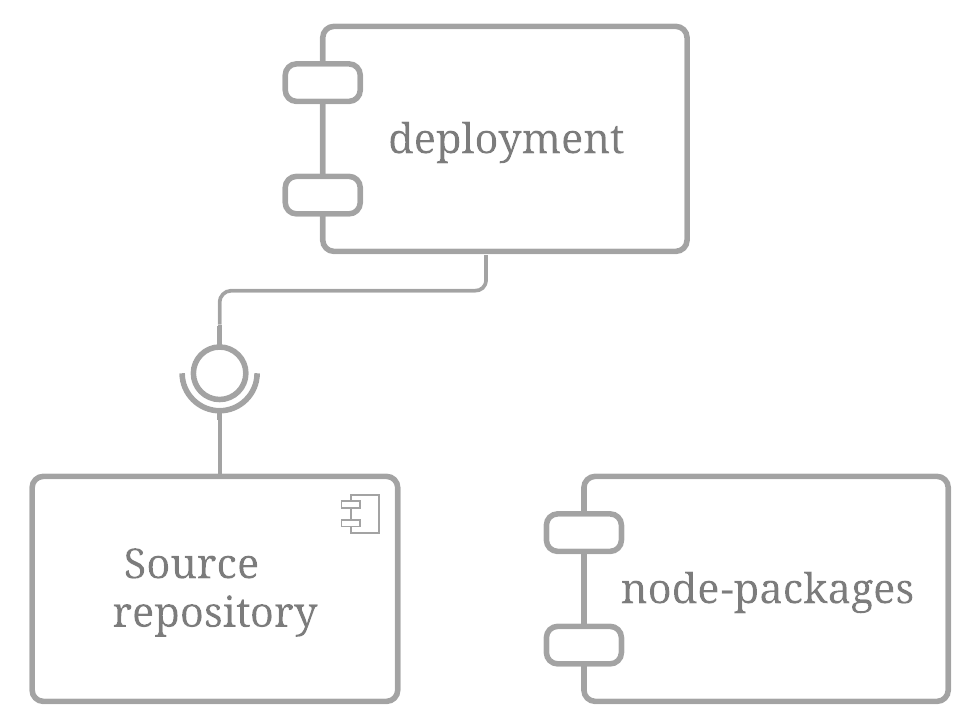
\includegraphics[scale=0.4]{src/figures/repository-components}
    \caption{Диаграмма компонентов репозиториев}
    \label{fig:repository-components}
\end{figure}

Таким образом, основными объектами в системе являются:
\begin{itemize}
    \item пользователь с набором прав доступа,
    \item репозиторий одного из типов,
    \item линия с задачами.
\end{itemize}

\section{Проектирование линий задач}

Для проектирования линий задач системы далее будет приведён разбор случаев использования с точки зрения CI/CD\cite{ciCd}.

В рамках данной работы ставится задача развернуть и настроить систему по автоматизации управления жизненным циклом веб-сервиса,
включающую автоматизированное тестирование компонентов веб-сервиса.

Основной целью такого тестирования является снижение количества ошибок в работе веб-сервиса и как следствие повышение соответствия к заявленным требованиям.
Данная цель будет достигаться при помощи двух основных линий, разделённых по виду тестирования и представленных в таблице \ref{tab:test-kinds}.

\begin{center}
    \begin{longtable}{|p{0.22\textwidth}|p{0.23\textwidth}|p{0.24\textwidth}|p{0.21\textwidth}|}
        \caption{Линии тестирования}
        \label{tab:test-kinds}
        \hline
        Название вида   & Условие запуска       & Местонахождение                               & Типы ошибок   \\
        \hline
        Модульное       & Каждый коммит         & Репозитории с исходным кодом                  & Семантические, компиляции, логические на уровне модуля    \\
        Интеграционное  & Каждый день в 10 утра & Репозиторий с конфигурациями развёртывания    & Логические на уровне веб-сервиса                          \\
        \hline
    \end{longtable}
\end{center}

Вследствие этого командой контроля качества были подготовлены автоматизированные тестовые сценарии.
Данные инструменты представляют консольные приложения на базе Node.js,
завершающихся с не нулевым кодом в случае нахождения ошибки.

\begin{itemize}
    \item проведение автоматизированного тестирования --- линия будет срабатывать на каждую синхронизацию с основной веткой удаленного репозитория и проводить разные виды тестирования,
    \item управление релизами сервиса и библиотек --- линия будет составляться в зависимости от ветки репозитория, собирать исходный код, загружать готовый к работе код в хранилище и
    оповещать кластер о выходе обновления при необходимости,
    \item управление развёрткой --- линия будет заключаться в применении обновлённых конфигураций окружения из репозитория к кластеру,
    \item получение доступа к исходному коду и хранилищам --- случай использования будет реализовываться не средствами CI/CD,
    \item сбор аналитических данных --- данные будут предоставляться артефактами в результате работы линий задач,
    \item управление правами доступа --- случай использования будет реализовываться не средствами CI/CD.
\end{itemize}

Самым частым этапом является проведение автоматизированного тестирования.
Так как система заранее не может знать о возможных сценариях использования веб-сервиса, то вся ответственность об их содержании переносится на тестировщика.
В целом, процесс тестирования будет происходить в несколько основных этапов: семантическое тестирование исходного кода, юнит и интеграционное тестирование библиотек и
определённых сервисов компонентов системы.
На основании данных этапов была составлена линия задач процесса тестирования веб-сервиса:

\begin{itemize}
    \item lint --- семантическое тестирование исходного кода путём запуска встроенного скрипта модуля разработчиками,
    \item test --- юнит и интеграционное тестирование библиотек веб-сервиса путём запуска скрипта модуля разработчиками и предоставление артефактов выполнения,
\end{itemize}

Создание релиза будет происходить похоже на создание релиза в git flow, только к комитам привязаны действия линий задач:
исполнение комита при помощи git, проведение тестирования, сборка образа и оповещение кластера.
На основании данных этапов была составлена линия задач создания релиза веб-сервиса:

\begin{itemize}
    \item test --- осуществление контроля качества путём запуска задач линии тестирования,
    \item build --- сборка исходного кода нужной версии и загрузкой в хранилище в зависимости от требуемого окружения (опциональная задача, требует подтверждения пользователем),
    \item publish --- оповещение кластера или зависимых сервисов о выходе обновления.
\end{itemize}

\begin{figure}[ht]
    \centering
    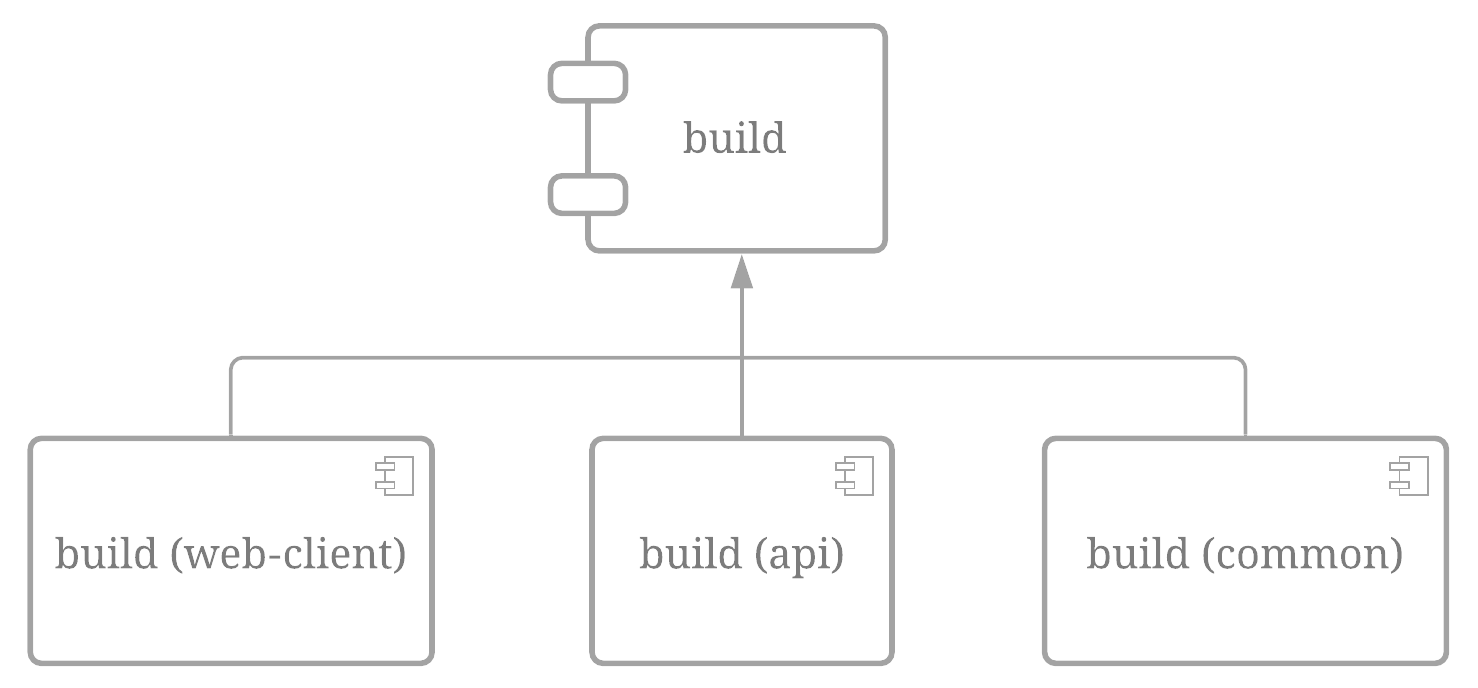
\includegraphics[scale=0.3]{src/figures/build-components}
    \caption{Диаграмма объектов стадии build}
    \label{fig:build-components}
\end{figure}

Данная линия будет иметь следующие аргументы:

\begin{itemize}
    \item название сервиса компонента, который необходимо обновить;
    \item название окружения, в котором необходимо произвести релиз.
\end{itemize}

Так как шаги сборки исходного кода и оповещения о релизе зависят лишь от входных инструкций Dockerfile, то данные шаги будут
скрыты от разработчиков веб-сервиса в репозитории с конфигурациями развёртывания.
Разработчику необходимо будет только импортировать необходимые задачи из репозитория.

Конфигурация развёртывания веб-сервиса состоит из линии, включающей только одну задачу: применение конфигураций развёртывания к кластеру.
В целях структуризации конфигураций для этих целей будет использоваться задача publish из линии по созданию релиза, которая при отсутствии аргументов будет обновлять конфигурации рахвёртки кластера.

\section{Выбор сервисов архитекутры}

Проводя обзор доступных на рынке git хостингов, можно сделать вывод, что наиболее распространенным git хостингом на сегодняшний день является хостинг компании GitLab Inc.
К тому же, по соотношению цена-функционал хостинг этой компании существенно обходит конкурентов.
Также, к существенному преимуществу можно отнести наличие обширного сообщества пользователей и разработчиков программных решений на основе git хостинга GitLab,
что позволяет иметь доступ к множеству готовых решений и получать помощь в разработке при необходимости.

Для реализации поставленной в данной работе задачи гибкость настройки всей инфраструктуры окружения не требуется, а также ставится в приоритет скорость ввода в рабочее состояние.
Поэтому в качестве оркестратора вместо гибкости Kubernetes был выбран Docker Swarm\cite{devOpsPhy}.
Но так как в данной работе делается акцент на гибкость всей системы, то далее будет рассмотрена описание конфигурации для использования с Kubernetes, не считая уставноку и настройку самого кластера.
Для работы будет подготовлена одна вершина Docker Swarm в статусе менеджер, поскольку более не требуется на данном этапе.

Одной и ключевой настройкой является открытие портов на уровне операционной системы сервера\cite{web:docker:swarm}:

\begin{itemize}
    \item TCP порт 2377 для коммуникации между менеджерами кластера,
    \item TCP и UDP порты 7946 для взаимодействия между нодами кластера,
    \item UDP порта 4789 для управления сетевым трафиком.
\end{itemize}

Как было сказано ранее, для развёртывания в работе используется Docker, поэтому необходим простой инструмент удалённого доступа к сокету Docker сервиса на рабочем сервере.
Для этих целей будет использоваться GitLab Runner с установленным исполнителем задач Docker.
Кратко описать работу GitLab Runner можно следующим образом: GitLab Runner запускается в отдельном контейнере с добавленным volume на сокет Docker,
таким образом получается избежать достаточно сложного и нецелесообразного запуска Docker внутри Docker,
так как в этом случае GitLab Runner получает доступ напрямую к сокету Docker сервера.

Данное решение имеет потенциальную проблему с безопасностью, поскольку если злоумышленник получит доступ к описанию задач GitLab CI/CD, то он сможет запускать на рабочем сервере любое ПО.
Для избежания данной проблемы будут установлены настройки доступа внутри GitLab.
Так же для избежания потери полезного времени работы GitLab Runner, необходимо будет произвести настройку кэша GitLab Runner.
Ключевой настройкой является политика загрузки образов для задач, поскольку по умолчанию GitLab Runner в любом случае будет загружать образ из регистра, даже если образ представлен локально.
Согласно требованиям GitLab Runner должен будет запускать минимум три задачи за единицу времени, данное значение будет отражено в конфигурации на этапе реализации.

\section{Подготовка плана тестирования}

Перед началом работы над планом сразу стоит отметить, что тестирование будет проводиться самим же разработчиком системы, что нарушает один из основных принципов тестирования.
Но в данном случае это оправдано, поскольку работа выполняет одним человеком.

Так же автор работы имеет доступ к исходному коду веб-сервиса и имеет открытый доступ к алгоритмам работы системы, что определяет метод тестирования --- белого ящика.

Основная цель проведения данного тестирования --- это снижение количества ошибок в работе линий и задач, а так же конфигурационных файлов.
Отсюда следует набор основных ошибок для нахождения при поведении тестирования: синтаксические в описании конфигураций и логические в работе линий и задач.
Так как GitLab предоставляет графический веб-интерфейс, то проведение тестирования на разных браузерах и операционных системах нецелесообразно,
поскольку сбор такого типа ошибок не удовлетворяет поставленной цели.

Ключевыми факторами, определяющими результат тестового сценария являются:
\begin{enumerate}
    \item репозиторий;
    \item хеш коммита в репозитории.
\end{enumerate}

Тестовый сценарий не может считаться пройденным или нет в случае, если GitLab Runner не отвечает на входящие запросы, поскольку это не содержит информации о результате выполнения линий задач,
но длительный простой задач в случае корректной работы линий свидетельствует о перегруженности сервера.

Основную часть синтаксических и логических ошибок можно найти и исправить на этапе описания файлов конфигураций, поскольку GitLab предоставляет удобный веб эмулятор GitLab Runner.
Использование данного эмулятора не поможет при поиске более сложных логических ошибок, поскольку задачи не будут исполняться, тем не менее его применение значительно ускоряет рабочий процесс разработки и описания файлов конфигураций.

\begin{figure}[ht]
    \centering
    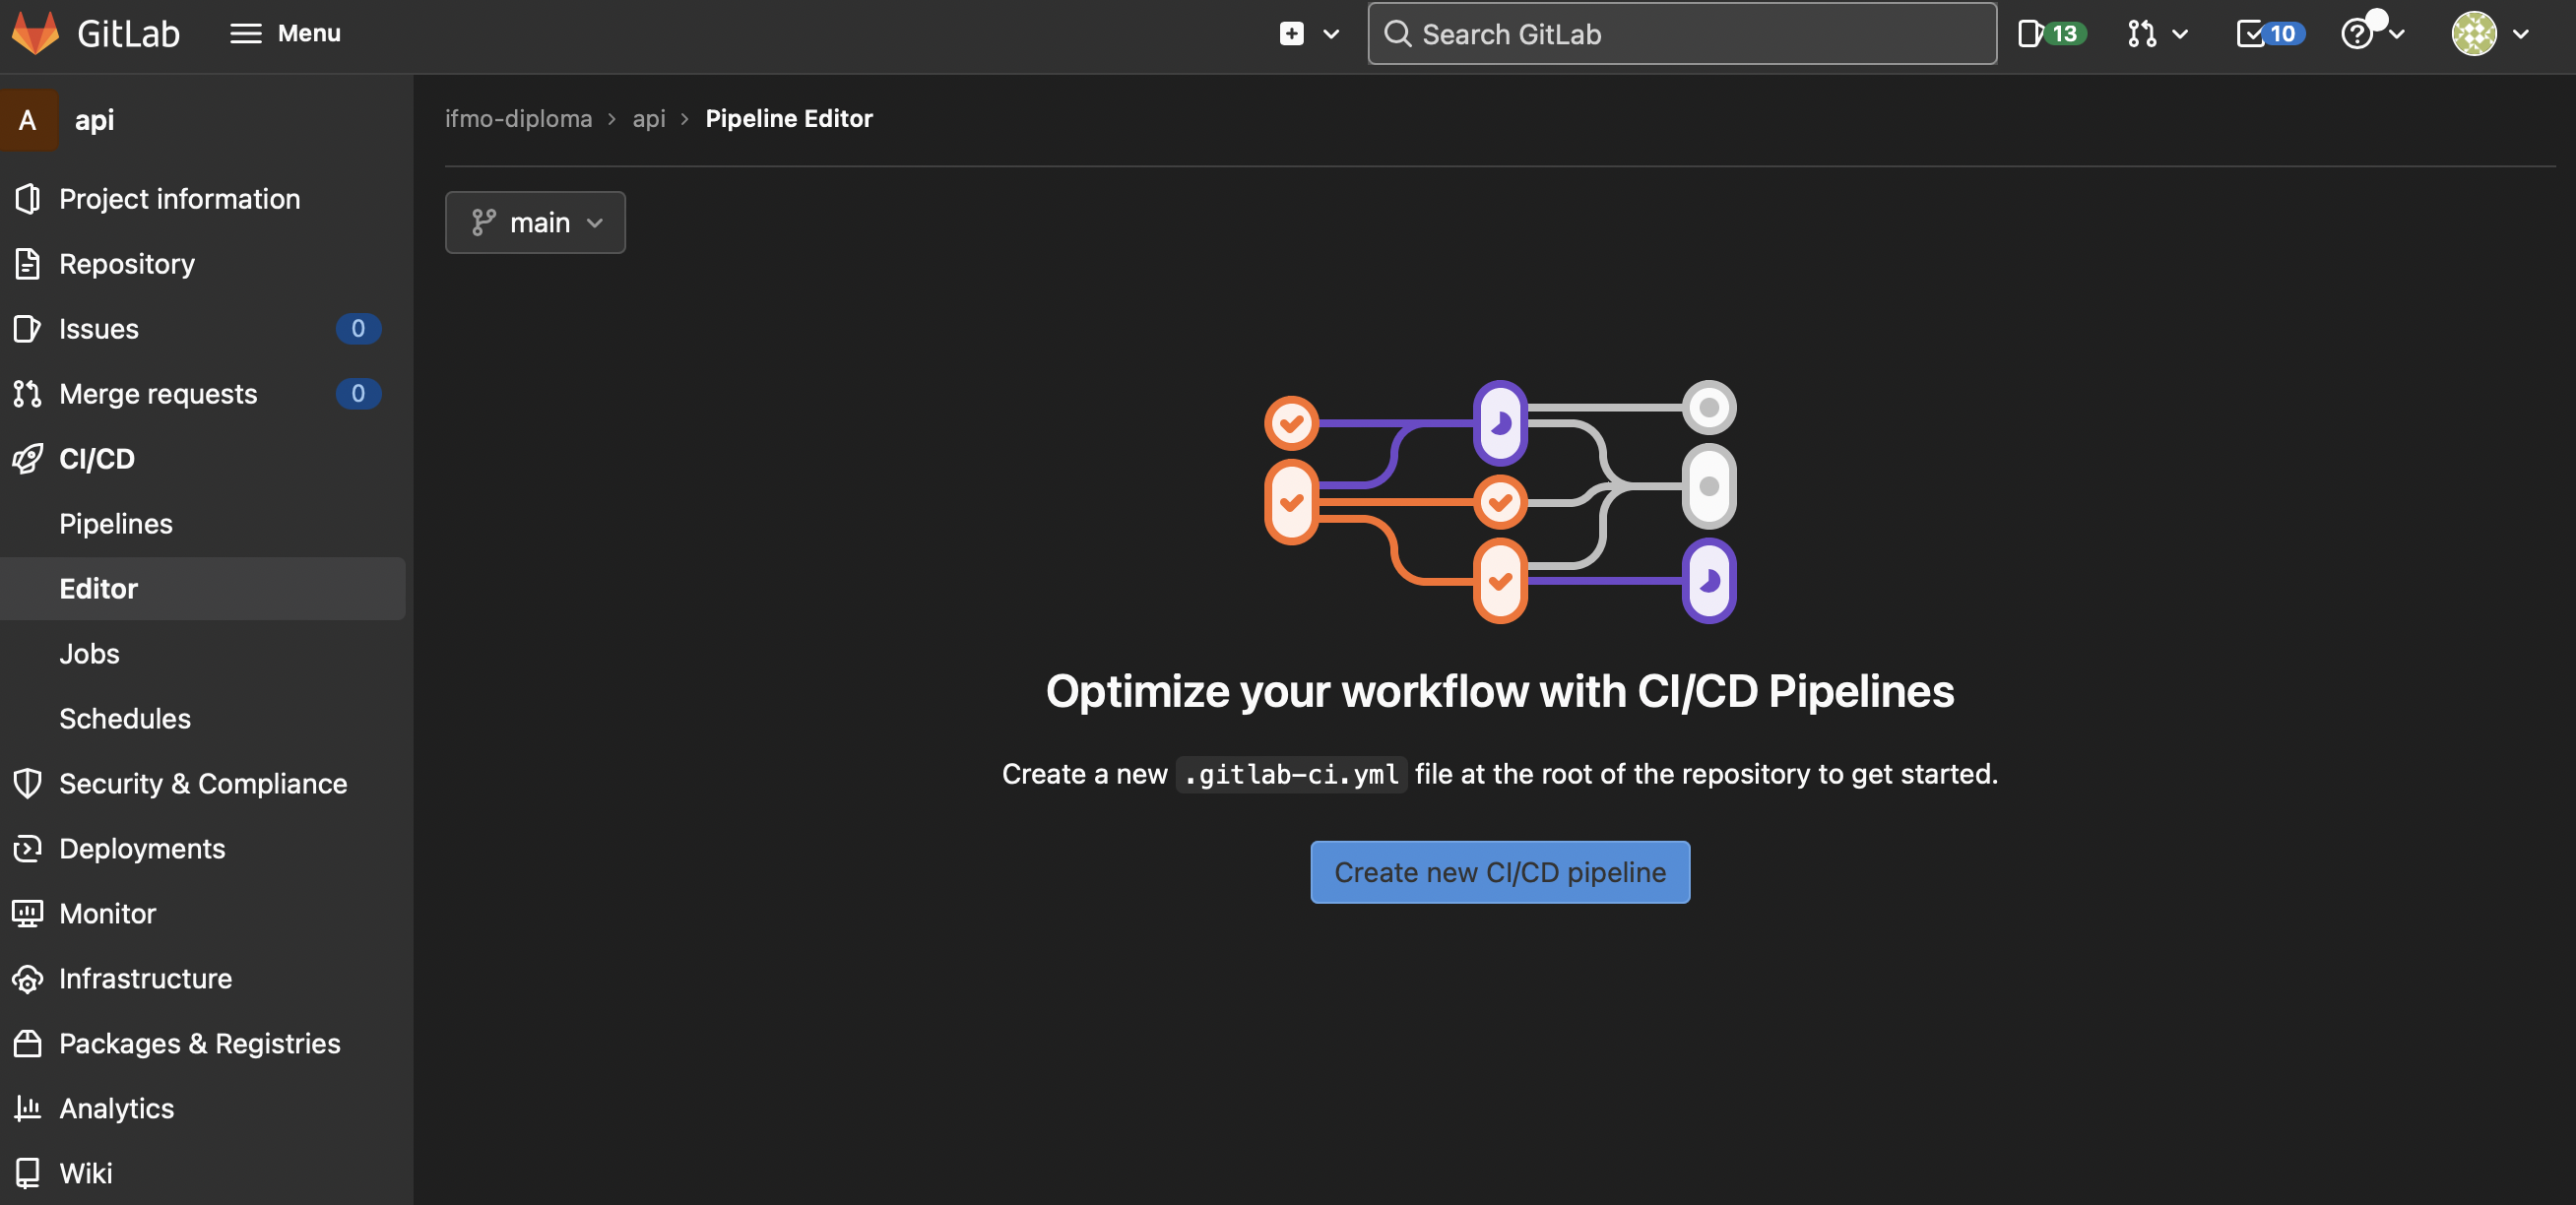
\includegraphics[scale=0.33]{src/figures/gitlab-editor}
    \caption{GitLab эмулятор линий и задач}
    \label{fig:gitlab-editor}
\end{figure}

Для нахождения и последующего исправления комплексных логических, требующих запуска задач, был составлен план тестирования в виде таблицы \ref{tab:testing-plan}.
Тестовые сценарии в плане основаны на случаях использования системы

\begin{center}
    \begin{longtable}{|c|p{0.15\textwidth}|p{0.2\textwidth}|p{0.2\textwidth}|p{0.2\textwidth}|}
        \caption{План тестирования}
        \label{tab:testing-plan}
        \hline
        № & Название тестового сценария             & Тестовый сценарий                                                                                         & Тестовые данные                           & Ожидаемый результат \\
        \hline
        1 & Линия задач автоматизации тестирования  & Открыть репозитории сервисов, проверить срабатывание и составление линий автоматизированного тестирования & Список сервисов компонентов веб-сервиса   & Линии собираются правильно, задачи выполняются, артефакты предоставляются \\
        \hline
        2 & Линия задач релиза создания релиза  & Открыть репозитории сервисов, проверить срабатывание и составление линий создания релиза & Список сервисов компонентов веб-сервиса   & Линии собираются правильно, задачи выполняются, веб-сервиса обновляется \\
        \hline
        3 & Линия задач управления развёрткой  & Открыть репозиторий развёртывания, изменить конфигурации развёртывания, зафиксировать изменения коммитом & Конфигурации развёртывания веб-сервиса   & Веб-сервис правильно реагирует на изменение конфигураций развёртывания \\
        \hline
    \end{longtable}
\end{center}

%%% Local Variables:
%%% mode: latex
%%% TeX-master: "rpz"
%%% End:
